\documentclass[french]{beamer}


%%% Style
%%% Gabarit de présentation du DMS
\RequirePackage{graphicx}
\usepackage{colortbl}


%%% Couleurs
\definecolor{bleu-udem}{RGB}{0, 107, 182}
\definecolor{gris-udem}{RGB}{102, 102, 102}
\definecolor{rouge}{RGB}{204, 0, 0}
\definecolor{vert}{RGB}{153, 204, 0}

\usecolortheme{lily}  % désinstalle les couleurs par défaut
\setbeamercolor*{normal text}{fg=black,bg=white}
\setbeamercolor*{alerted text}{fg=rouge}
\setbeamercolor*{example text}{fg=vert}
\setbeamercolor*{structure}{fg=black}

\setbeamercolor*{block title}{fg=white,bg=gris-udem}
\setbeamercolor*{block title alerted}{fg=white,bg=gris-udem}
\setbeamercolor*{block title example}{fg=white,bg=gris-udem}

\setbeamercolor*{block body}{bg=black!10}
\setbeamercolor*{block body alerted}{bg=black!10}
\setbeamercolor*{block body example}{bg=black!10}

\setbeamercolor{item}{fg=bleu-udem}
\setbeamercolor{background canvas}{bg=gris-udem!5}


%%% Liens
\hypersetup{
  colorlinks=true,
  pdfnewwindow=true,
  linkcolor=gris-udem,
  citecolor=bleu-udem,
  filecolor=bleu-udem,
  urlcolor=bleu-udem
}


%%% Canva
\newlength{\textmarginL}
\newlength{\textmarginR}
\setlength{\textmarginL}{7.5mm}
\setlength{\textmarginR}{3.5mm}
\setbeamersize{text margin left=\textmarginL, text margin right=\textmarginR}
\newlength{\titleseparator}
\setlength{\titleseparator}{.71\paperwidth}  % distance entre le côté gauche et la barre horizontale (Page titre)
\newenvironment{changemargin}[2]{%
  \begin{list}{}{%
    \setlength{\topsep}{0pt}%
    \setlength{\leftmargin}{#1}%
    \setlength{\rightmargin}{#2}%
    \setlength{\listparindent}{\parindent}%
    \setlength{\itemindent}{\parindent}%
    \setlength{\parsep}{\parskip}%
  }%
  \item[]}{\end{list}}

%%% Images et logo
\newcommand{\insertslidelogo}{\rule{0pt}{.14\paperheight}} % .14\paperheight = .22\paperwidth
\newcommand{\slidelogo}{
  \renewcommand{\insertslidelogo}{
	
\includegraphics[height=.14\paperheight]{figures/logos/mila}
  }
}
\newcommand{\inserttitlelogo}{\rule{0pt}{.16\paperheight}}  % .16\paperheight = .25\paperwidth
\newcommand{\titlelogo}{
  \renewcommand{\inserttitlelogo}{
	
\includegraphics[height=.16\paperheight]{figures/logos/mila}
  }
}
\newcommand{\inserttitleimage}{\rule{0pt}{.28\paperheight}}
\newcommand{\titleimage}[1]{
  \renewcommand{\inserttitleimage}{
  \includegraphics[height=.28\paperheight, keepaspectratio=true]{#1}
  }
}


%%% Page titre
\setbeamertemplate{title page}{
\begin{changemargin}{-\textmarginL}{-\textmarginR}
\begin{tabular}{@{}r!{\color{bleu-udem}\vline}@{}l@{}}
 & \inserttitlelogo\\
\inserttitleimage & \\
\rule{0pt}{20pt}
\parbox{\titleseparator}{\flushright\Large{\inserttitle}} & \\
\parbox{\titleseparator}{\flushright\small{\insertsubtitle}}  & \\
\rule{0pt}{24pt}
\parbox{\titleseparator}{\flushright\insertauthor} & \\
\parbox{\titleseparator}{\flushright\insertinstitute}  & \\
\rule{0pt}{18pt}
\parbox{\titleseparator}{\flushright\small{\insertdate}} & \\
\end{tabular}
\end{changemargin}
}


%%% Entête
\setbeamertemplate{frametitle}{%
\vskip-33pt\parbox[c]{.68\paperwidth}{\large\insertframetitle}\vskip4pt%
}
\setbeamertemplate{headline}{%
\hfill\insertslidelogo

\color{bleu-udem}\rule{.98\paperwidth}{.07pt}%
}


%%% Pied de page
\beamertemplatenavigationsymbolsempty
\newcommand{\numsubsectionname}{}
\newcommand{\showsubsection}{
  \renewcommand{\numsubsectionname}{%
	\thesection.\thesubsection \; \insertsubsection
  }
}
\newcommand{\insertfootlinetext}{}
\newcommand{\footlinetext}[1]{
  \renewcommand{\insertfootlinetext}{#1}
}
\setbeamertemplate{footline}{
{\hfill\color{bleu-udem}\rule{.98\paperwidth}{0.07pt}}%
\vskip4pt%
\color{gris-udem}%
\rule{0.02\paperwidth}{0pt}%
\numsubsectionname
\hfill%
\mbox{\insertfootlinetext\qquad\qquad\insertframenumber}%
\rule{\textmarginR}{0pt}%
\vskip4pt%
}



%%% Extensions utiles pour le français
\usepackage[french]{babel}
\usepackage[utf8]{inputenc}
\usepackage[T1]{fontenc}

\usepackage{xcolor}
\usepackage{setspace}

%%% Extensions utiles pour les math
\usepackage{amsmath}
\usepackage{amsfonts}
\usepackage{bbold}
\usepackage{mathtools}

\DeclareMathOperator*{\argmin}{arg\,min}

%%% Extensions pour les figures
\usepackage{graphicx}
\usepackage{subfig}
\usepackage{tikz}

%%% Bibliographie
\usepackage{bibentry}

%%% Informations sur la présentation
\author{Patrice Béchard}
\institute[MILA]{\small{MILA}}
% please come up with a better title
\title{Comprendre le langage humain}
\subtitle{Approches neuronales}
\date{\today}


%%% Préférences (Propre au thème du DMS)
\slidelogo
\titlelogo
\titleimage{figures/seq2seq.png}  % Image à afficher sur la page titre
\footlinetext{  % À utiliser surtout pour les congrès
\insertshorttitle\quad\insertshortdate\quad\insertshortinstitute
}


\def\signed #1{{\leavevmode\unskip\nobreak\hfil\penalty50\hskip2em
  \hbox{}\nobreak\hfil(#1)%
  \parfillskip=0pt \finalhyphendemerits=0 \endgraf}}

\newsavebox\mybox
\newenvironment{aquote}[1]
  {\savebox\mybox{#1}\begin{quote}}
  {\signed{\usebox\mybox}\end{quote}}

\usepackage{ragged2e}


%%% Début
\begin{document}


\begin{frame}[plain, t]
  \titlepage
\end{frame}

%%% Context

\begin{frame}{Mise en contexte}

\centering
{\LARGE Pourquoi le traitement des langues naturelles?}
\vspace{.5cm}

\raggedright
\begin{itemize}
	\item Énormément de données disponible en ligne sous forme textuelle.
	\vspace{.5cm}
	\item On veut faire plusieurs choses avec cette information :
	\begin{itemize}
		\item Résumer pour trouver l'information importante
		\item Traduire automatiquement d'une langue à une autre
		\item Détecter le sentiment des utilisateurs d'un produit
		\item Avoir une réponse à une question
		\item etc.
	\end{itemize}
\end{itemize}
\end{frame}

%%% Definition : NLP

\begin{frame}{Traitement automatique des langues naturelles}

\centering
{\LARGE C'est quoi le traitement des langues naturelles?}
\vspace{.5cm}

\raggedright
\begin{itemize}
	\item Branche de l'intelligence artificielle visant la compréhension du langage.
	\item Natural Language Processing/Understanding (NLP/NLU)
	\item On y compte des tâches telles que :
	\begin{itemize}
		\item Résumés automatiques de texte
		\item Traduction automatique
		\item Analyse de sentiments
		\item Systèmes de question et réponse
		\item Agents conversationnels
		\item Reconnaissance vocale
		\item etc.
	\end{itemize}
\end{itemize}
\end{frame}

%%% Table of contents

\begin{frame}{Plan de l'exposé}
  \tableofcontents
\end{frame}

%%% Introduction to machine learning

\section{Bases de l'apprentissage automatique}

\begin{frame}{}
\centering
{\Huge Bases de \\ l'apprentissage automatique}
\end{frame}

\begin{frame}{Bases de l'apprentissage automatique}
\textbf{Deux approches à l'intelligence artificielle}
\vspace{0.5cm}

\begin{columns}[T] % align columns
\begin{column}{.48\textwidth}
\begin{center}
\underline{IA «classique» symbolique}
\end{center}
\begin{itemize}
	\item Fondé sur le \\raisonnement logique
	\item Règles codées à la main \\(\texttt{if... else...})
	\item Pas de gestion de l'incertain
\end{itemize}

\end{column}%
\hfill%
\begin{column}{.48\textwidth}
\begin{center}
\underline{Apprentissage automatique}
\end{center}
\begin{itemize}
	\item Apprendre les paramètres à partir d'exemples
	\item Approche probabiliste
	\item Objectif : \textbf{généralisation}
\end{itemize}
\end{column}%
\end{columns}
\end{frame}

\begin{frame}{Bases de l'apprentissage automatique}
\textbf{Types de problèmes}
\vspace{0.5cm}

\begin{itemize}
	\item Apprentissage supervisé
	\begin{itemize}
		\item Régression
		\item Classification
	\end{itemize}
	\item Apprentissage non-supervisé
	\begin{itemize}
		\item Réduction de dimensionalité, clustering, détection d'anomalie, ...
	\end{itemize}
	\item Apprentissage par renforcement
\end{itemize}
\end{frame}

\begin{frame}{Bases de l'apprentissage automatique}
\textbf{Apprentissage supervisé}
\vspace{0.5cm}
\begin{itemize}
	\item Ensemble de données $\mathcal{D_{\mathrm{train}}} = \{(x^{(1)}, y^{(1)}), (x^{(2)}, y^{(2)}), \dots,  (x^{(N)}, y^{(N)})\}$.
	\item Le modèle prédit une sortie $f(x^{(i)})$ en fonction de l'entrée $x^{(i)}$. On veut que le modèle prédise la cible $y^{(i)}$.
	\item Lors de la phase d'entraînement, le modèle ajuste ses paramètres $\Theta$ dans le but de minimiser le risque empirique $\hat{R}$ selon une fonction de coût $\mathcal{L}(y, f(x))$
\end{itemize}
$$
\hat{R} = \frac{1}{N} \sum_{i=1}^N \mathcal{L}\left(y^{(i)}, f(x^{(i)})\right)
\qquad
\Theta^* = \argmin_\Theta \hat{R}(f, \mathcal{D}_{train})
$$
\end{frame}

\begin{frame}{Bases de l'apprentissage automatique}
\textbf{Quelques fonctions de coût...}
\vspace{.5cm}
\begin{itemize}
	\item Erreur quadratique (régression) : 
	\vspace{-.2cm}
	$$ \mathcal{L}(y, f(x)) = ||y-f(x)||_2^2$$
	\item Erreur de classification : 
	\vspace{-.2cm}
	$$\mathcal{L}(y, f(x)) = \mathbb{1}_{\{y \neq f(x) \}}$$
	\item Entropie croisée binaire : 
	\vspace{-.2cm}	
	$$ \mathcal{L}(y, f(x)) = -y \log f(x) + (1-y) \log (1-f(x))$$
	\item Moins log-vraisemblance : 
	\vspace{-.2cm}	
	$$ \mathcal{L}(y, f(x)) = - \log f(x)_y $$
\end{itemize}
\end{frame}

\begin{frame}{Bases de l'apprentissage automatique}
\textbf{Estimer l'erreur de généralisation}
\vspace{.5cm}
\begin{itemize}
	\item But de l'apprentissage machine : \textbf{généralisation}
	\item On test le modèle entraîné sur des exemples jamais vus auparavant :
	\vspace{-.2cm}
	$$\mathcal{D}_{\mathrm{test}} = \{ (x^{(1')}, y^{(1')}), (x^{(2')}, y^{(2')}), \dots, (x^{(N')}, y^{(N')}) \}$$
\end{itemize}
\begin{center}
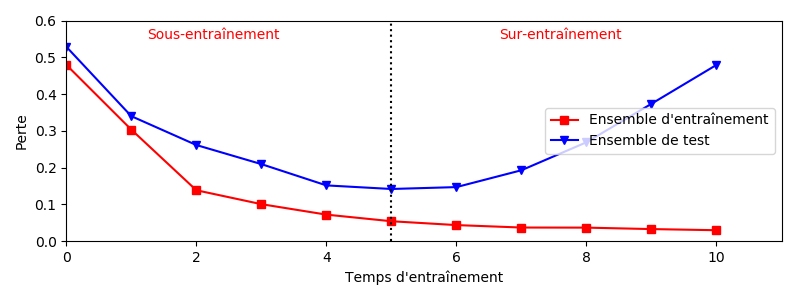
\includegraphics[height=3.5cm]{figures/learning_curve}
\end{center}
\end{frame}

\begin{frame}{Bases de l'apprentissage automatique}
\textbf{Exemple : Prédiction du prix des maisons à Boston \cite{harrison1978hedonic}}
\vspace{0.5cm}
\begin{columns}[T] % align columns
\begin{column}{.48\textwidth}
\begin{itemize}
	\item Problème de régression
	\item \textbf{Entrée} : 13 traits caractéristiques ($\in \mathbb{R}^{13}$)\\ ex: Nb. de chambres, Taux de criminalité, ...
	\item \textbf{Sortie} : Prix de la maison ($\in \mathbb{R}$)
\end{itemize}
\end{column}%
\hfill%
\begin{column}{.48\textwidth}
\centering
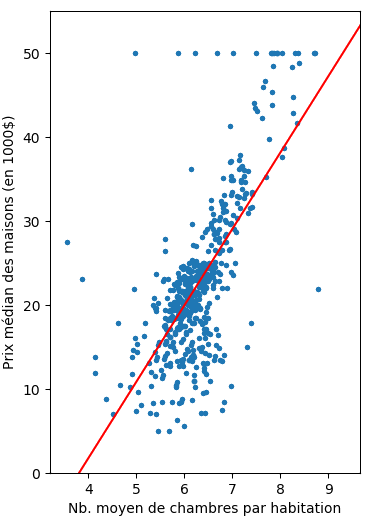
\includegraphics[height=6cm]{figures/boston}
\end{column}%
\end{columns}
\end{frame}

\begin{frame}{Bases de l'apprentissage automatique}
\vspace{0.5cm}
\textbf{Exemple : Classification de chiffres manuscrits \cite{lecun1998mnist}}
\begin{itemize}
	\item Problème de classification
	\item Entrée : Image 28x28 px
	\item Sortie : Chiffre de 0 à 9
\end{itemize}
\vspace{0.5cm}
\begin{center}

\includegraphics[height=3cm]{figures/mnist-2}
\end{center}
\end{frame}


% Reseaux de neurones et apprentissage profond

\section{Réseaux de neurones et apprentissage profond}

\begin{frame}{}
\centering
{\Huge Réseaux de neurones et \\ apprentissage profond}
\end{frame}

\begin{frame}{Réseaux de neurones et apprentissage profond}
\begin{columns}[T]
\begin{column}{.48\textwidth}
\begin{center}
\underline{Neurone biologique}\\
\vspace{.5cm}
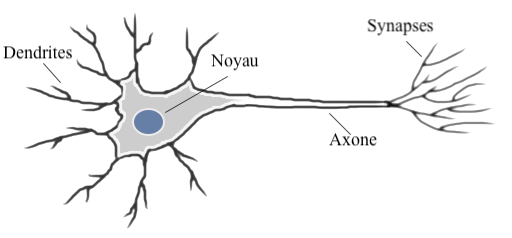
\includegraphics[width=\linewidth]{figures/biological_neuron}
\end{center}
\end{column}
\hfill
\begin{column}{.48\textwidth}
\begin{center}
\underline{Neurone artificiel}\\
\vspace{.5cm}
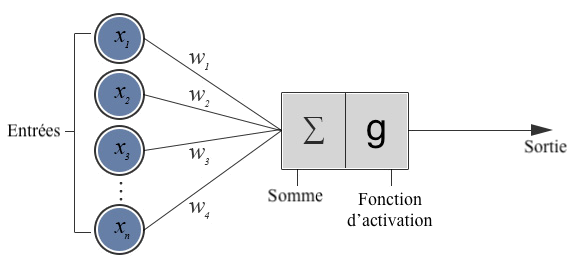
\includegraphics[width=\linewidth]{figures/artificial_neuron}
\end{center}
\end{column}
\end{columns}
\end{frame}

\begin{frame}{Réseaux de neurones et apprentissage profond}
\textbf{Quelques fonctions d'activation}
\vspace{-.5cm}
\begin{columns}[T]
\begin{column}{.48\textwidth}
\begin{center}
\underline{Linéaire} : $g(x) = x$\\
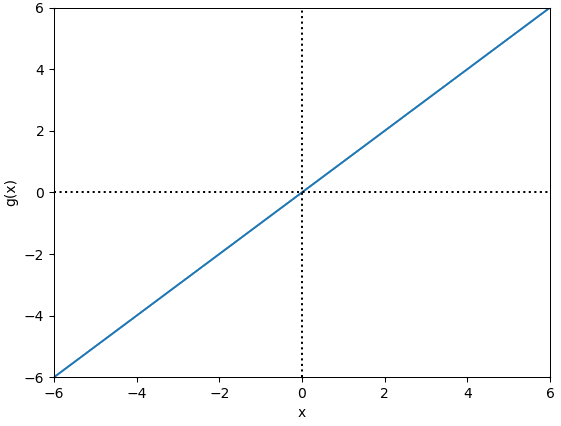
\includegraphics[width=.6\linewidth]{figures/linear}\\
\underline{ReLU} : $g(x) = max(0, x)$\\
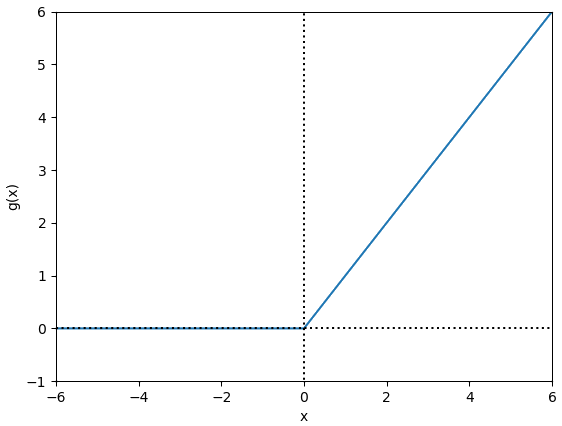
\includegraphics[width=.6\linewidth]{figures/relu}\\
\end{center}
\end{column}
\hfill
\begin{column}{.48\textwidth}
\begin{center}
\underline{Sigmoïde} : $g(x) = \frac{1}{1 + \exp (-x)}$\\
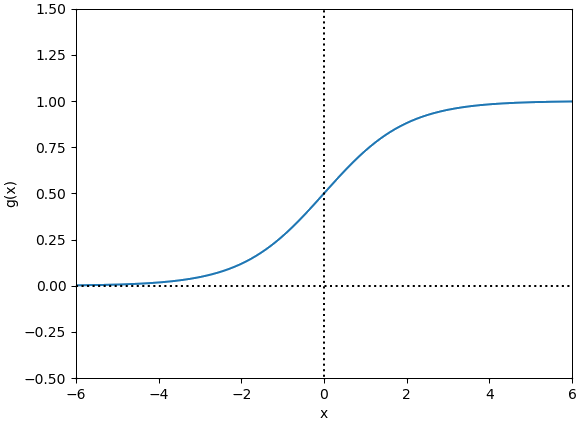
\includegraphics[width=.6\linewidth]{figures/sigmoid}\\
\underline{Tanh} : $g(x) = \tanh(x)$\\
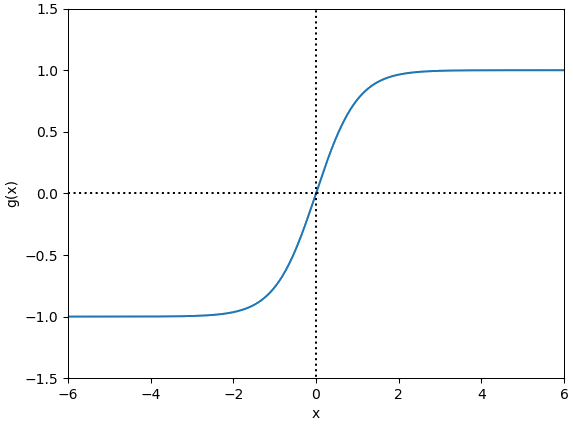
\includegraphics[width=.6\linewidth]{figures/tanh}
\end{center}
\end{column}
\end{columns}
\end{frame}

% Modeles lineaires
\subsection{Modèles linéaires}

\begin{frame}{Réseaux de neurones et apprentissage profond}
\textbf{Modèle linéaire : Régression linéaire}
\vspace{0.5cm}
\begin{itemize}
	\item Modèle pour la régression
\end{itemize}
$$ f(\mathrm{x}) = \mathrm{w}^T\mathrm{x} + b = \sum_i \mathrm{w}_i \mathrm{x}_i + b $$
Représentation neuronale :\\
\centering
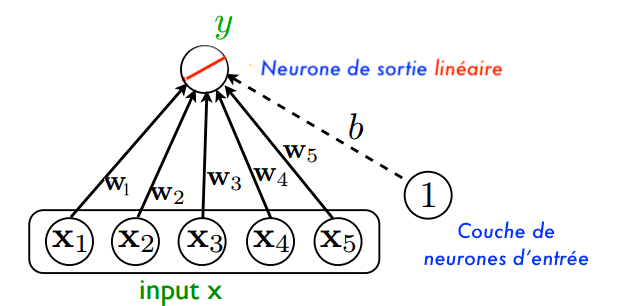
\includegraphics[height=3cm]{figures/linear_regression}
\end{frame}

\begin{frame}{Réseaux de neurones et apprentissage profond}
\textbf{Modèle linéaire : «Régression» logistique}
\vspace{0.5cm}
\begin{itemize}
	\item Modèle pour la classification binaire
\end{itemize}
$$ f(\mathrm{x}) = \mathrm{sigm}\left( \mathrm{w}^T\mathrm{x} + b \right) = \mathrm{sigm}\left( \sum_i \mathrm{w}_i \mathrm{x}_i + b \right) $$
Représentation neuronale :\\
\centering
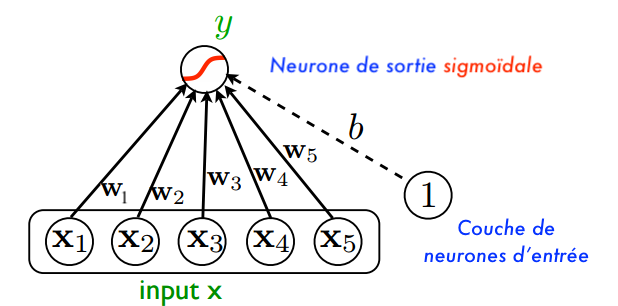
\includegraphics[height=3cm]{figures/logistic_regression}
\end{frame}

\begin{frame}{Réseaux de neurones et apprentissage profond}
\textbf{Problème : ensembles de données non linéairement séparables}
\vspace{-.5cm}
\begin{columns}[T]
\hfill
\begin{column}{.3\textwidth}
\begin{center}
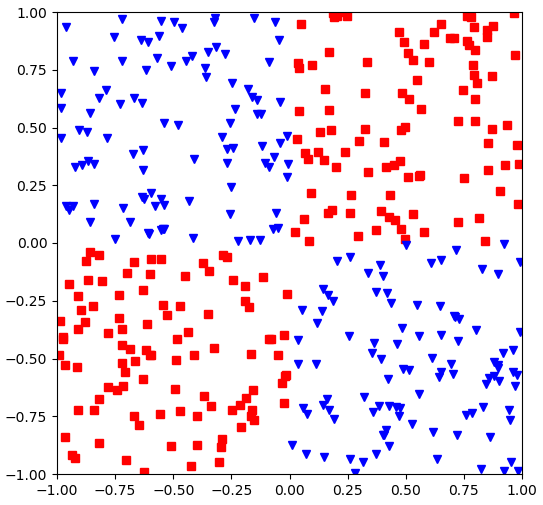
\includegraphics[width=\linewidth]{figures/xor} \\
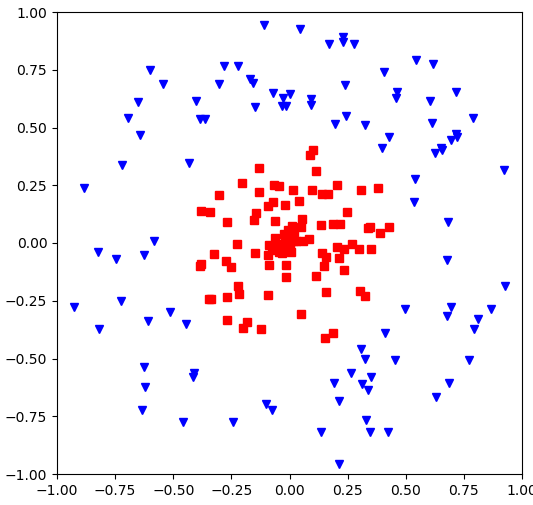
\includegraphics[width=\linewidth]{figures/circle}
\end{center}
\end{column}
\pause
\begin{column}{.3\textwidth}
\vspace{1.5cm}
$$\xrightarrow[\text{deux composantes}]{\text{Multiplier les}}$$
\vspace{2cm}
$$ \xrightarrow[\text{polaires}]{\text{Coordonnées}} $$
\end{column}
\begin{column}{.3\textwidth}
\begin{center}
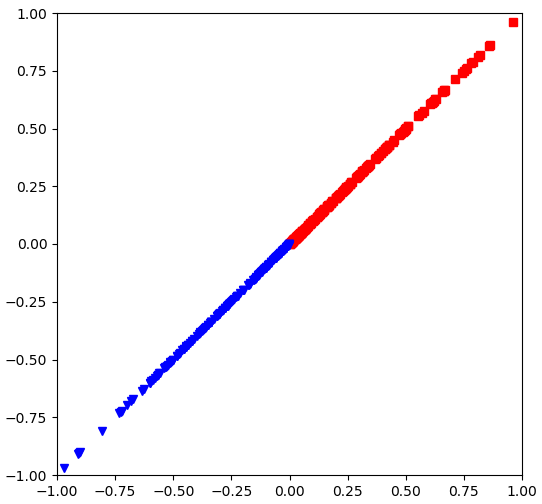
\includegraphics[width=\linewidth]{figures/xor_transform} \\
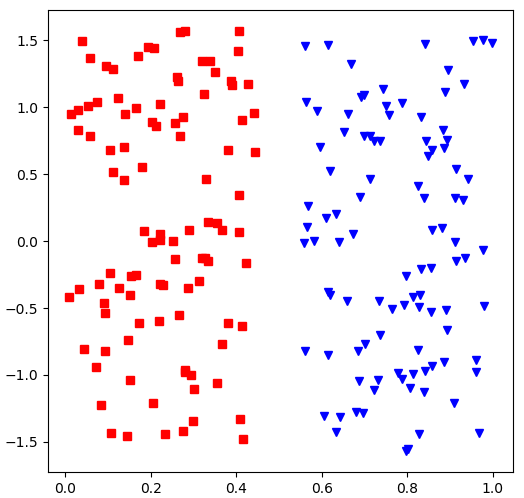
\includegraphics[width=\linewidth]{figures/circle_transform} \\
\end{center}
\end{column}
\hfill
\end{columns}
\end{frame}

%%% Multi Layer Perceptron

\subsection{Perceptron multicouche}

\begin{frame}{Réseaux de neurones et apprentissage profond}
\begin{center}
{\Large Comment définir ces nouvelles représentations pour chaque ensemble de données?} \\
\pause
\vspace{1cm}
{\Large{\textcolor{red}{On laisse le modèle les apprendre!}}}
\end{center}
\end{frame}

\begin{frame}{Perceptron multicouche (MLP)}
\textbf{Introduction d'une couche de neurones cachés}

\begin{columns}[T]
\begin{column}{.48\textwidth}
\begin{itemize}
	\item Entrée : $\mathrm{x} \in \mathbb{R}^d$
	\item Paramètres : \\ $W^{(1)} \in \mathbb{R}^{d\times d_h}$, $b^{(1)} \in \mathbb{R}^{d_h}$ \\ $W^{(2)} \in \mathbb{R}^{d_h \times d_o}$, $b^{(2)} \in \mathbb{R}^{d_o}$
	\item Propagation : \\ {\small $h^{(1)}\left(\mathrm{x}) = g^{(1)}(W^{(1), T}\mathrm{x} + b^{(1)}\right)$} \\ {\small$f(\mathrm{x})~=~g^{(2)}\left(W^{(2), T} h^{(1)}(\mathrm{x})~+~b^{(2)}\right)$}
\end{itemize}
\end{column}
\hfill
\begin{column}{.48\textwidth}
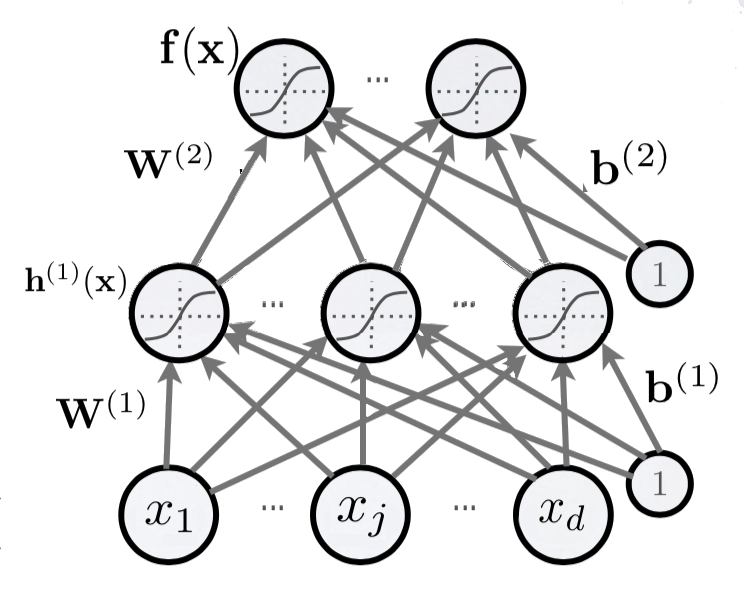
\includegraphics[width=\textwidth]{figures/nn}
\end{column}
\end{columns}
\end{frame}

\begin{frame}{Perceptron multicouche (MLP)}
\textbf{On peut aussi avoir plus d'une couche cachée!}
\begin{columns}[T]
\begin{column}{.48\textwidth}
\begin{itemize}
	\item C'est ce qu'on appelle l'\textbf{apprentissage profond}.
	\item Le nombre de couches cachées ainsi que le nombre de neurones dans chaque couche cachée sont des \textbf{hyperparamètres} que l'utilisateur doit ajuster manuellement
\end{itemize}
\end{column}
\hfillÒ
\begin{column}{.48\textwidth}
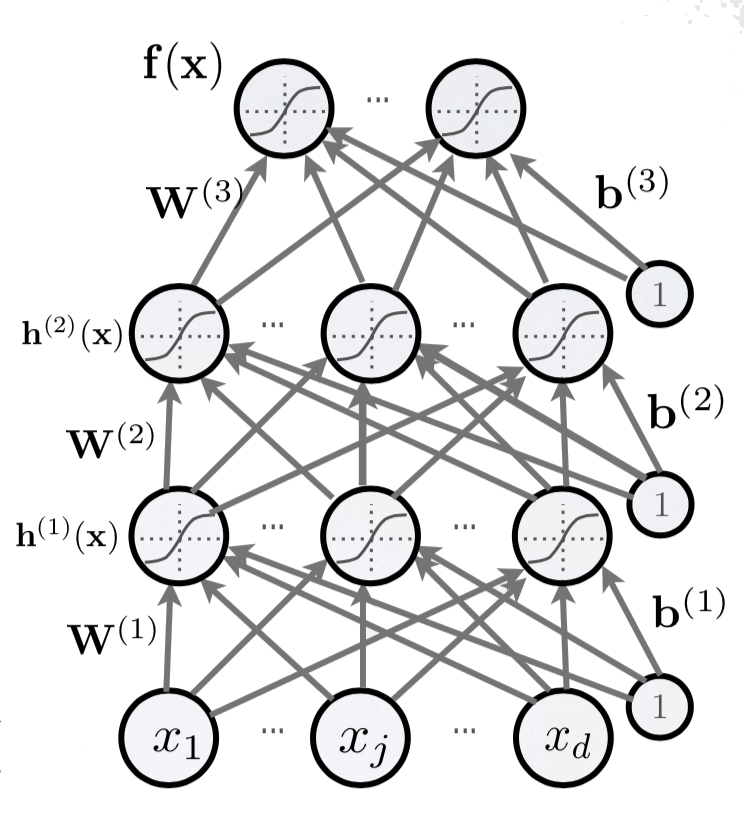
\includegraphics[width=\textwidth]{figures/deep_nn}
\end{column}
\end{columns}
\end{frame}

\begin{frame}{Perceptron multicouche (MLP)}
\textbf{Apprentissage des paramètres : algorithme de rétropropagation\cite{rumelhart1985learning}}
\begin{columns}[T]
\begin{column}{.52\textwidth}
{\small
\begin{itemize}
	\item On calcule le gradient de la fonction de coût $\nabla \mathcal{L}(f(x), y)$ pour chaque élément du réseau en utilisant la règle de dérivée en chaîne.
	\item On ajuste les paramètres dans la direction opposée du gradient : \\ $$ \theta^{(t+1)} \leftarrow \theta^{(t)} - \eta \nabla_{\theta}\mathcal{L}(f(x), y)^{(t)} $$
	\item Le \textbf{taux d'apprentissage} $\eta$ est un hyperparamètre à déterminer.
	\item On répète pour chaque exemple jusqu'à convergence.
\end{itemize}
}
\end{column}
\hfill
\begin{column}{.52\textwidth}
\only<1>{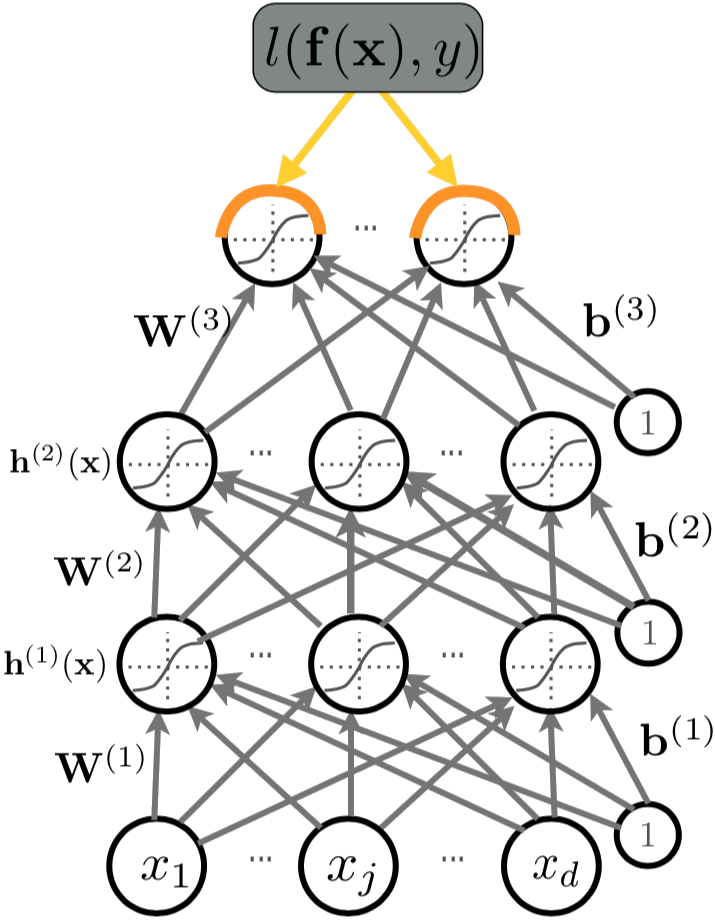
\includegraphics[width=.8\textwidth]{figures/backprop/1}}
\only<2>{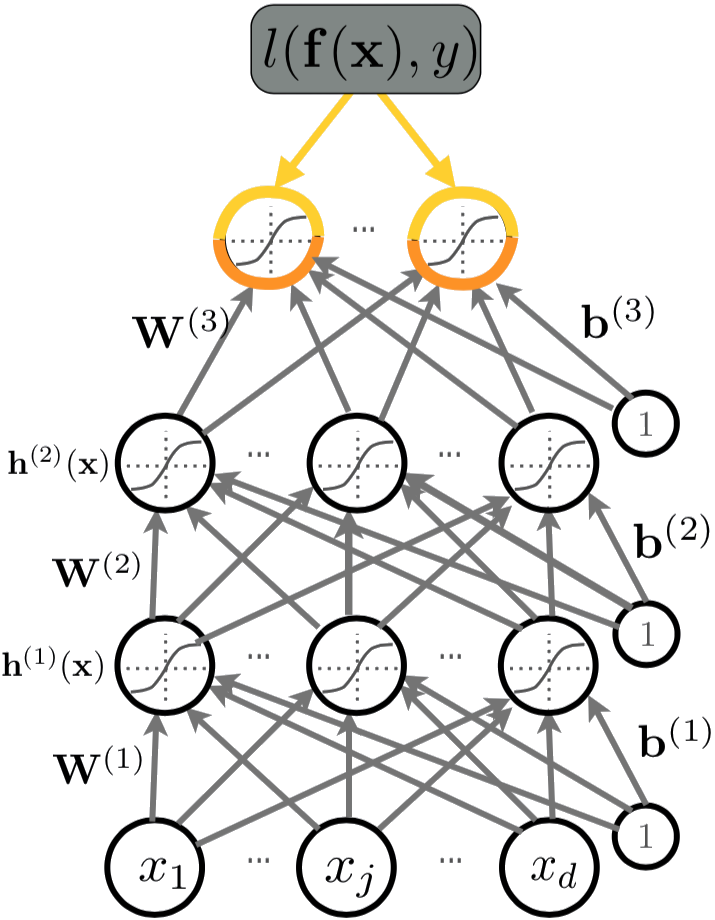
\includegraphics[width=.8\textwidth]{figures/backprop/2}}
\only<3>{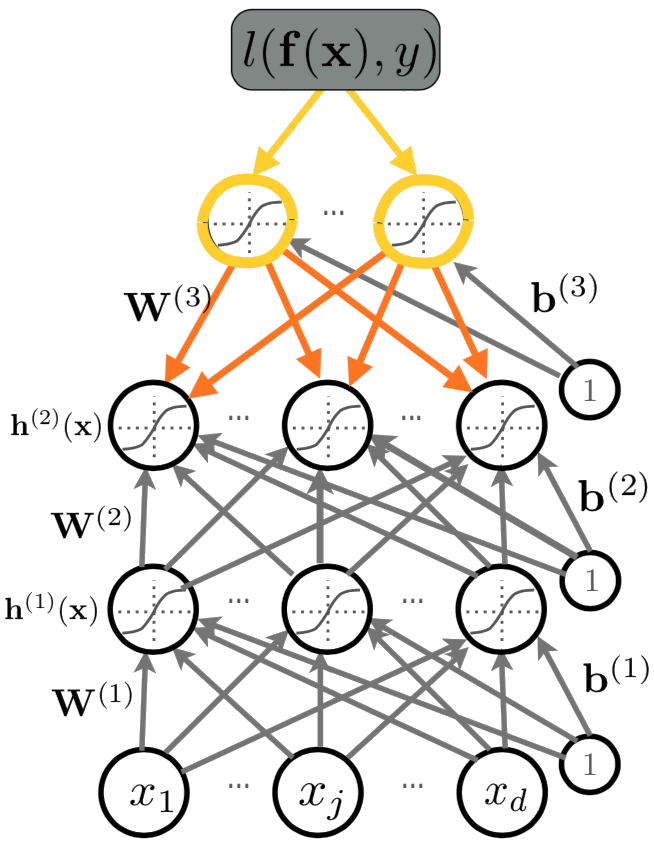
\includegraphics[width=.8\textwidth]{figures/backprop/3}}
\only<4>{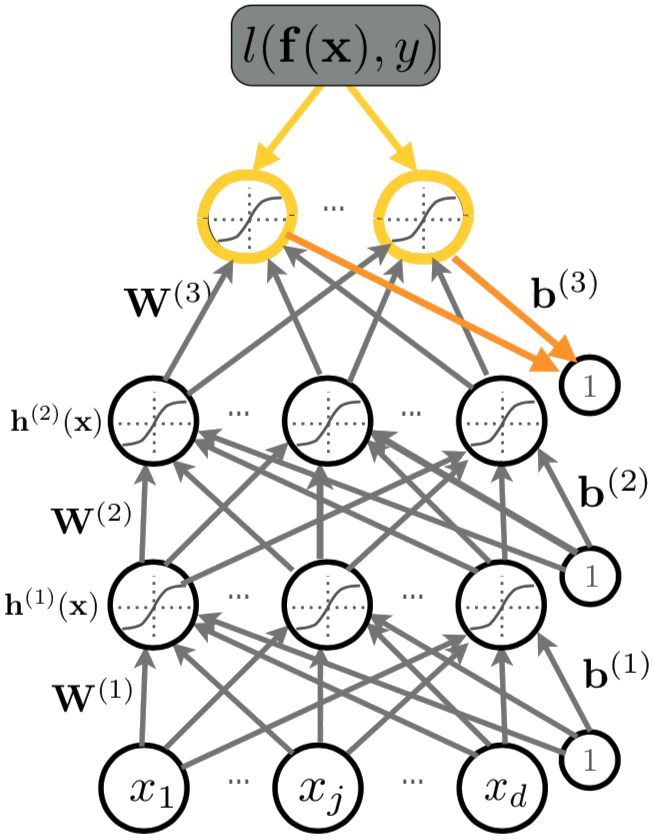
\includegraphics[width=.8\textwidth]{figures/backprop/4}}
\only<5>{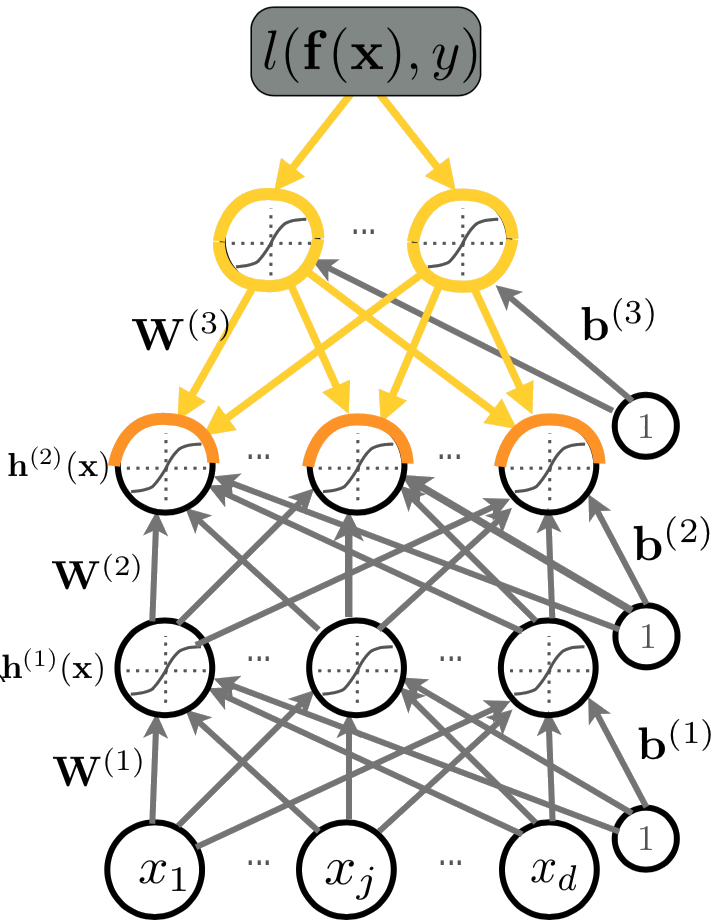
\includegraphics[width=.8\textwidth]{figures/backprop/5}}
\only<6>{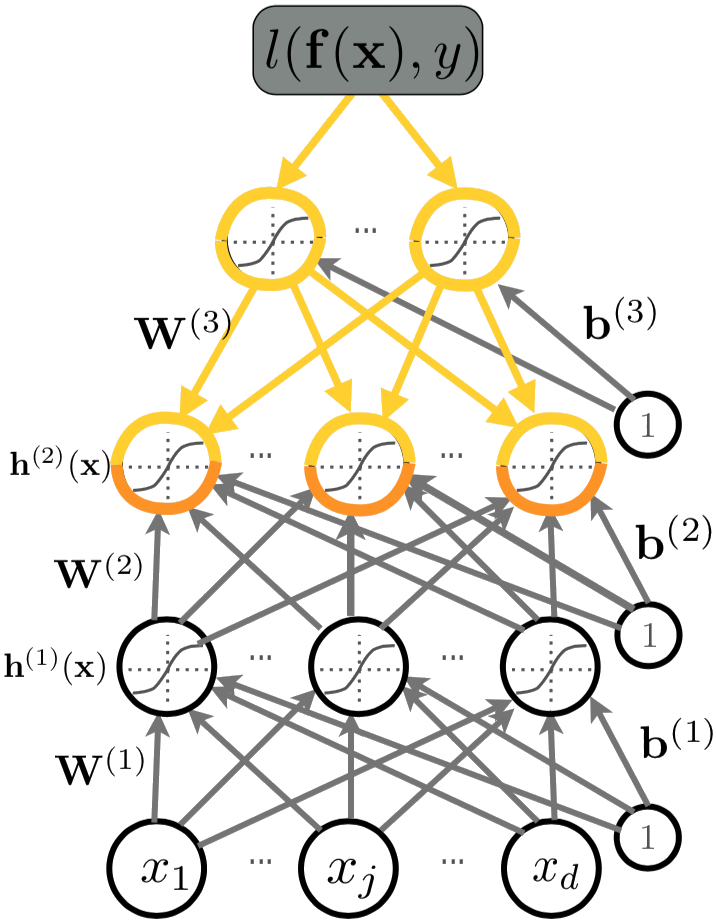
\includegraphics[width=.8\textwidth]{figures/backprop/6}}
\end{column}
\end{columns}
\end{frame}

% RNN

\subsection{Réseaux de neurones récurrents}

\begin{frame}{Réseaux de neurones récurrents (RNN)}
\begin{itemize}
	\item Utilisé dans les données avec corrélation temporelle et dans le traitement des langues naturelles
	\item Capable de manipuler des entrées de différentes longueurs
	\item Limitations : Difficulté avec les dépendances à long-terme
\end{itemize}

\centering
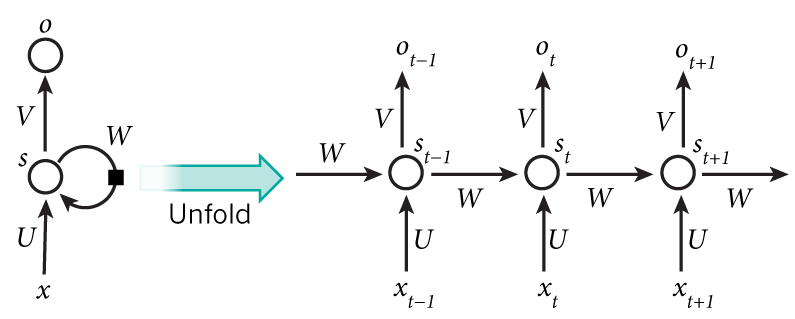
\includegraphics[width=.8\textwidth]{figures/rnn}

\raggedright
\cite{karpathy2015unreasonable} pour une excellente introduction aux RNN

\end{frame}

\begin{frame}{Réseaux de neurones récurrents (RNN)}
\begin{itemize}
	\item Solution : \textit{Long Short-Term Memory} (LSTM) \cite{hochreiter1997long}
	\item Permet au signal de se propager plus facilement dans le temps.
\end{itemize}

\centering
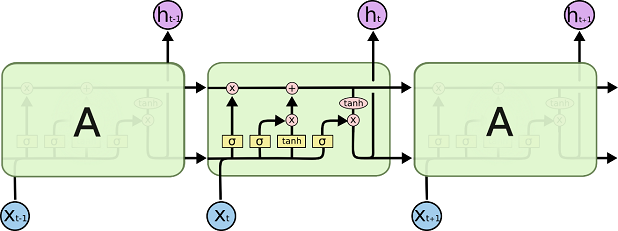
\includegraphics[width=.8\textwidth]{figures/lstm}

\raggedright
\cite{olah2015understanding} pour une excellente introduction aux LSTM

\end{frame}

\subsection{Modèles séquence à séquence}

\begin{frame}{Modèles séquence à séquence (Seq2Seq)\cite{cho2014learning}\cite{sutskever2014sequence}}
\begin{itemize}
	\item Permet de transformer une séquence de longueur arbitraire en autre séquence de longueur arbitraire
\end{itemize}
\begin{center}
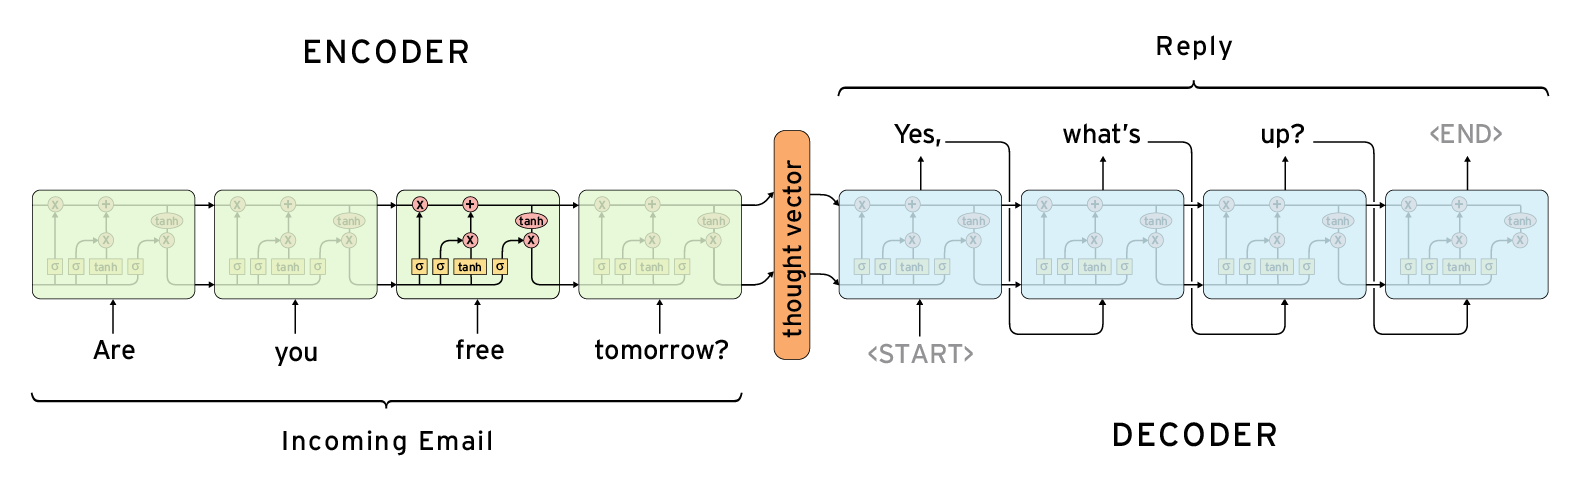
\includegraphics[width=\textwidth]{figures/seq2seq}
\end{center}
\end{frame}

%%% Representation des mots

\section{Bien représenter les mots}

\begin{frame}{}

\centering
{\Huge Bien représenter les mots}

\end{frame}

\begin{frame}{Bien représenter les mots}
\begin{itemize}
	\item Façon la plus simple : Vecteur \textit{onehot}
	\item Vecteur de dimension $V$ où tous les éléments sont $0$ sauf un élément qui est $1$.
	\item $V$ : Taille du vocabulaire
\end{itemize}

\vspace{.5cm}
Exemple : \\ 
\centering
\textbf{\large le chat est mignon .}

\vspace{.5cm}
\raggedleft
\begin{itemize}
	\item \textbf{chat} $\rightarrow [0, 1, 0, ..., 0, 0]$
\end{itemize}
\end{frame}

% Bag of Words

\subsection{Sac de mots}

\begin{frame}{Sac de mots}

\centering
{\Large Approche \textbf{Sac de mots} (Bag of Words)}
\vspace{.5cm}

\raggedright
Pour représenter un texte, on peut simplement additionner les vecteurs :

\begin{itemize}
	\item \textbf{le chat est mignon . } $ \rightarrow [0, 1, 1, 0, ..., 0, 1, 0, 1, 0, ... 0, 1]$
\end{itemize}

\end{frame}

\begin{frame}{Sac de mots}

Problèmes avec cette approche :
\begin{itemize}
	\item Beaucoup d'espace mémoire perdue. (La majorité des composantes du vecteur sont $0$)
	\item On pert l'ordre des mots avec cette représentation.
\end{itemize}
\centering
\textbf{"le chat mange la pizza ."} $=$ \textbf{"la pizza mange le chat ."}

\raggedleft
\begin{itemize}
	\item Tous les mots sont indépendants les uns des autres.
\end{itemize}
\centering
\textbf{chat} $\perp$ \textbf{chien}

\end{frame}

% Word Embeddings

\subsection{Word embeddings}

\begin{frame}{Word Embeddings}

\centering
{\Large Solution possible : \textbf{Word Embeddings} \cite{bengio2003neural}\cite{mikolov2013efficient}}
\vspace{.5cm}

\raggedright
On projette les vecteurs onehot dans un espace de dimension réduite. On \textbf{apprend} cette représentation
\vspace{.5cm}

2 approches dominantes :
\begin{itemize}
	\item \textit{Continuous Bag of Words (CBOW)}
	\item \textit{Skip-Gram}
\end{itemize}

\end{frame}

\begin{frame}{Word Embeddings}
\textbf{Continuous Bag of Words (CBOW)}
\begin{itemize}
	\item On utilise une fenêtre de contexte du mot et on essaie de prédire celui-ci.
\end{itemize}
\centering
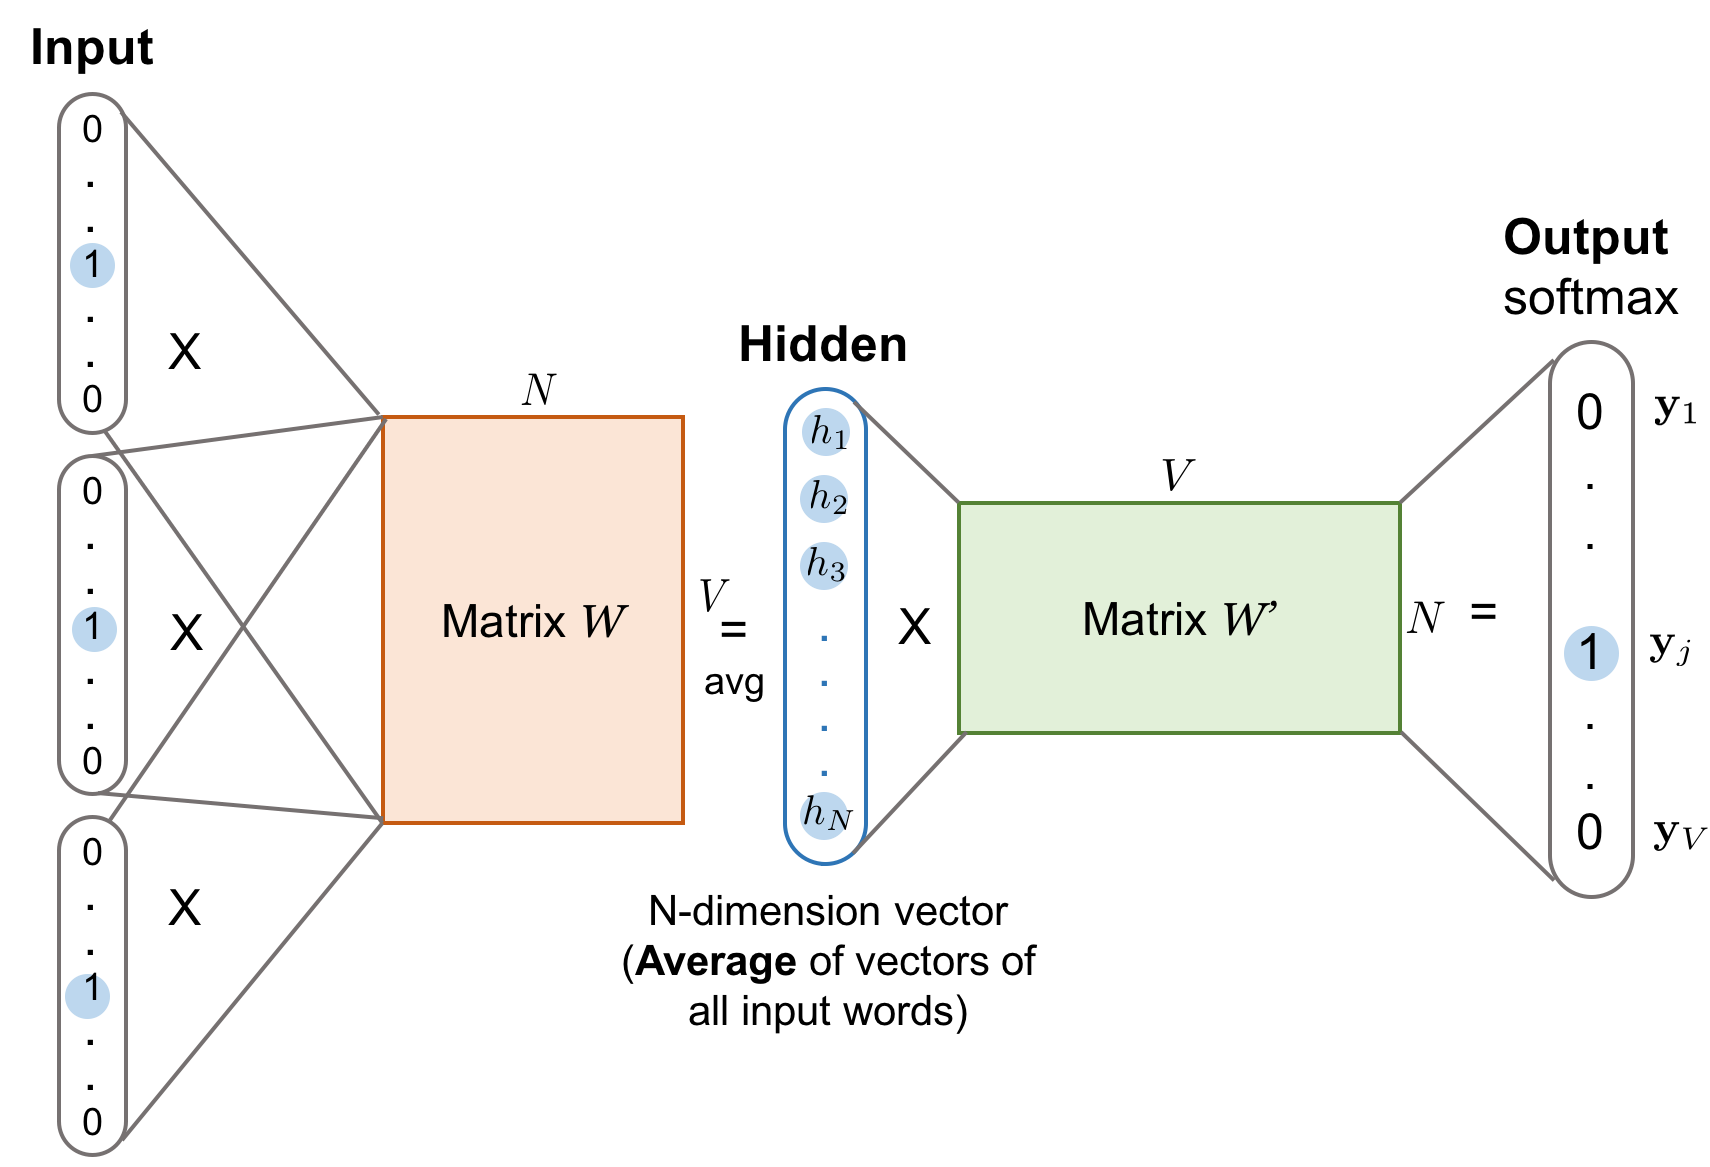
\includegraphics[height=6cm]{figures/word2vec-cbow.png}
\end{frame}

\begin{frame}{Word Embeddings}
\textbf{Skip-Gram}
\begin{itemize}
	\item On utilise le mot et on essaie de prédire son contexte.
\end{itemize}
\centering
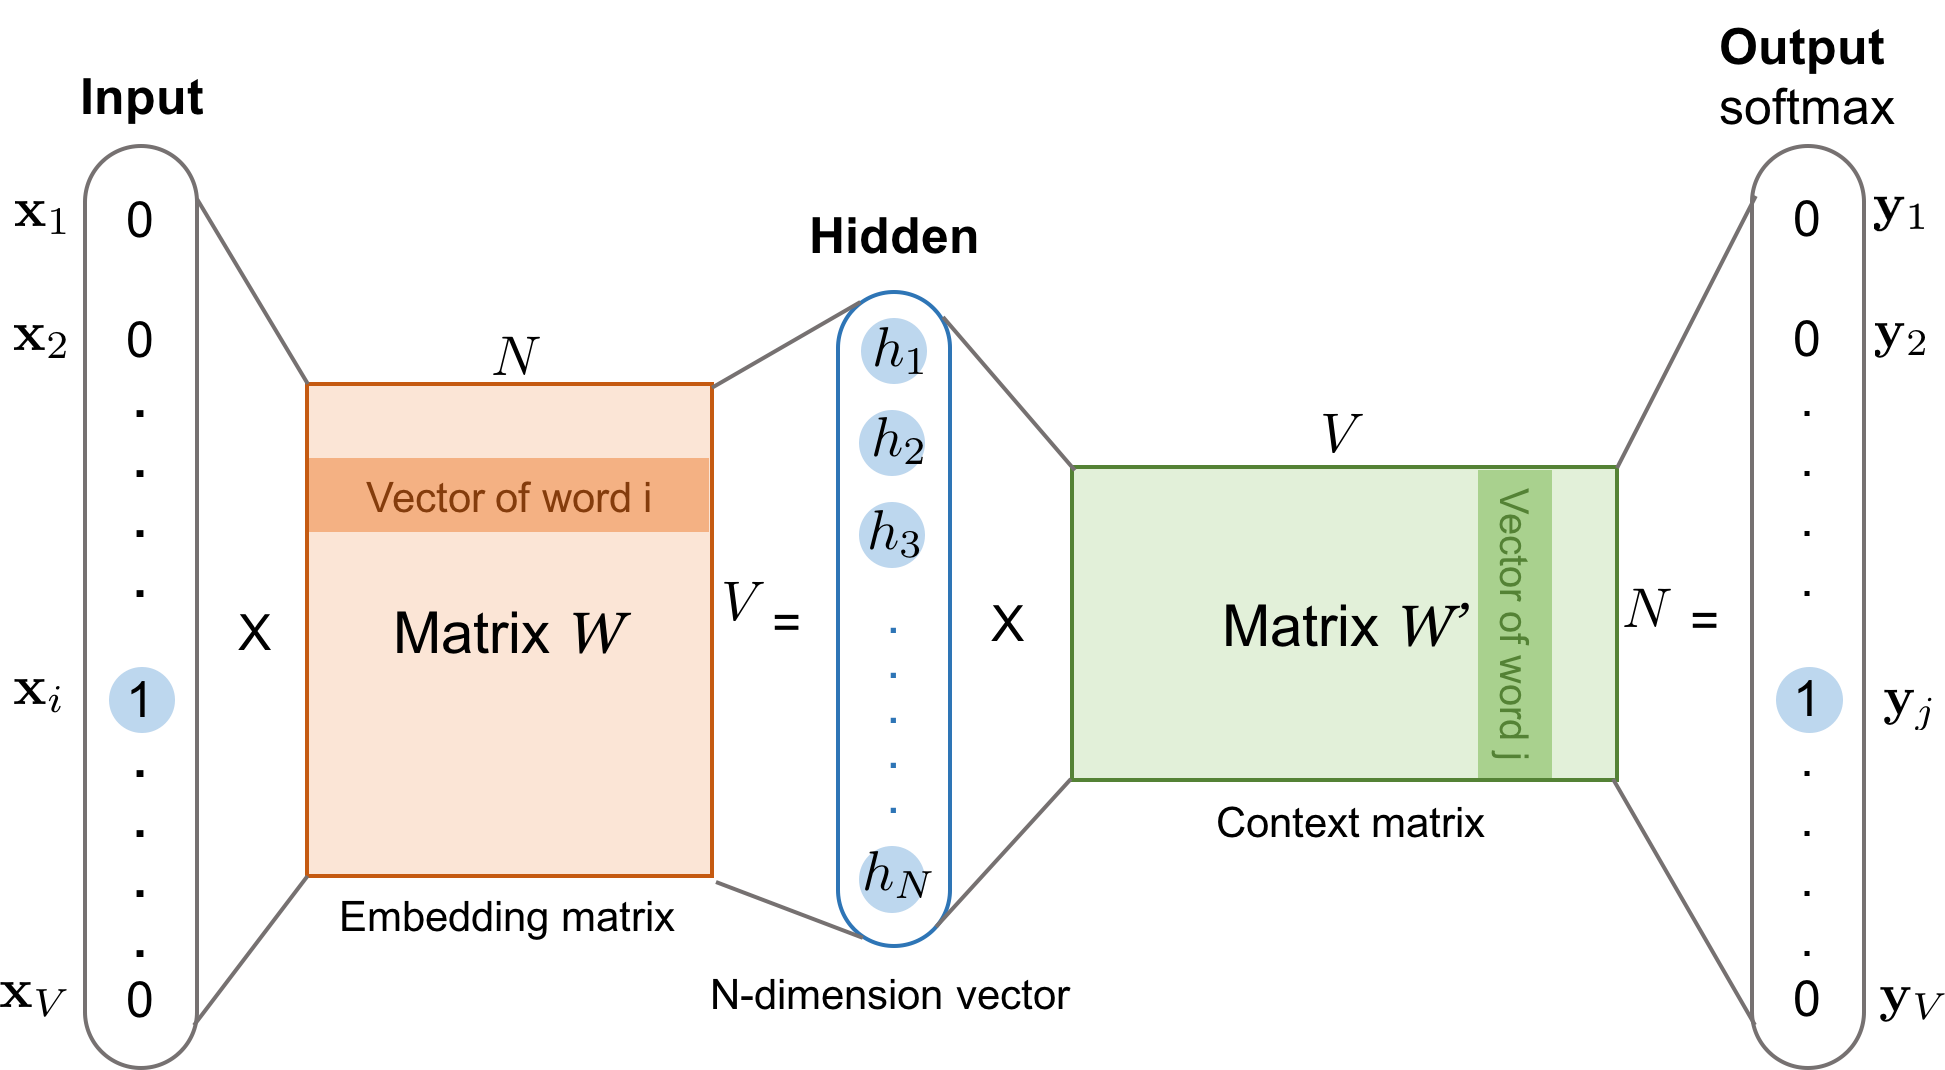
\includegraphics[height=6cm]{figures/word2vec-skip-gram.png}
\end{frame}

\begin{frame}{Word Embeddings}
$$ \mathrm{Repr(man)} - \mathrm{Repr(woman)} + \mathrm{Repr(King)} \approx \mathrm{Repr(Queen)} $$
\centering
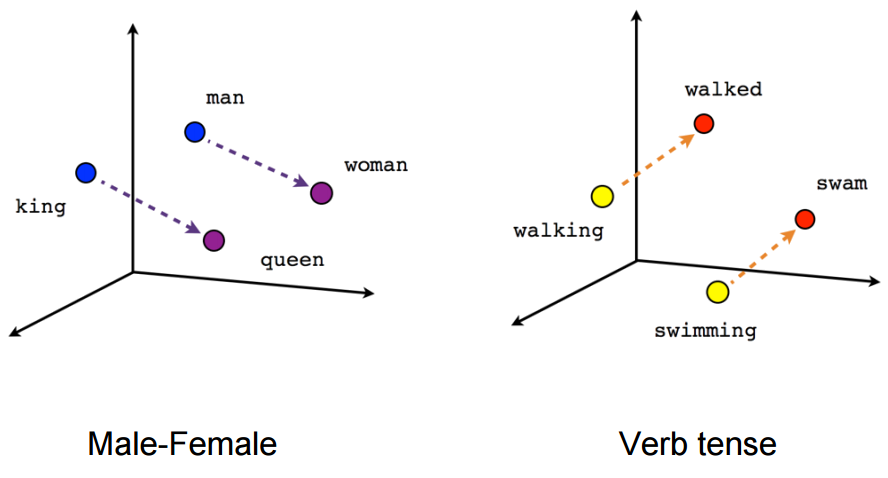
\includegraphics[height=6cm]{figures/male_female_verb_tense.png}

\end{frame}

\begin{frame}{Word Embeddings}
\centering
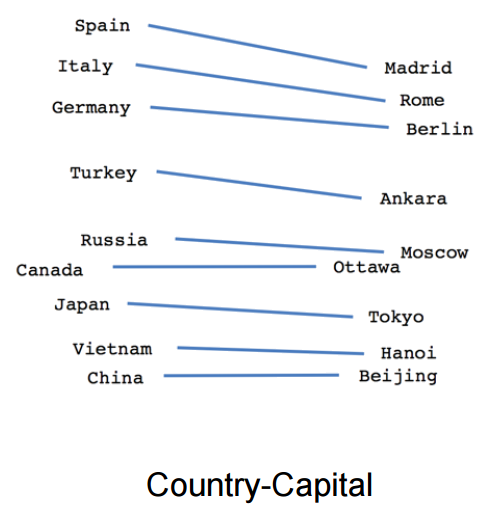
\includegraphics[height=6cm]{figures/capital_country.png}

\end{frame}

%%% Tâches en NLP

\section{Tâches en NLP}

\begin{frame}{}

\centering
{\Huge Quelques tâches en NLP}

\end{frame}

% Sentiment Analysis

\subsection{Analyse de sentiments}

\begin{frame}{Analyse de sentiments}

\begin{description}
	\item [Tâche] Prédire le sentiment véhiculé dans un texte.
	\item [Exemple] Prédire si une critique de film est positive ou négative.
\end{description}

\centering
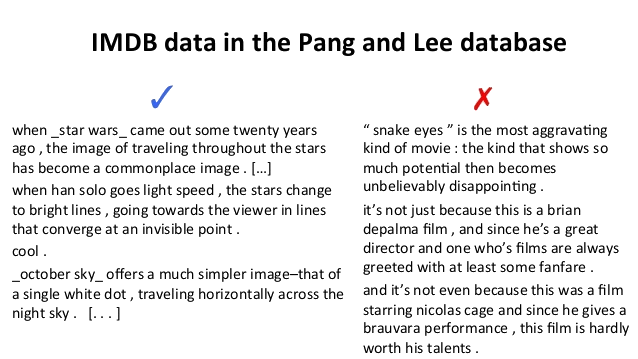
\includegraphics[height=6cm]{figures/sentiment_analysis_imdb.png}

\end{frame}

\begin{frame}{Analyse de sentiments}

Approche simple : \\
\begin{itemize}
	\item On représente le texte d'entrée avec l'approche Bag of Words.
	\item On utilise un MLP pour prédire une cible binaire
	\item 1 : positif, 0 : négatif
	\item \textbf{Résultats} : environ 88\% de bonnes réponses
\end{itemize}

\centering
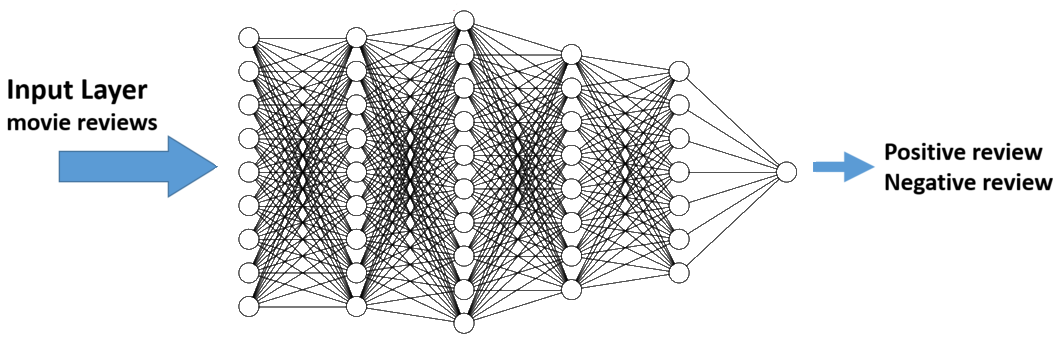
\includegraphics[width=\textwidth]{figures/sentiment_analysis_mlp.png}
\end{frame}

% RNN Language Model

\subsection{Modèles de langue}

\begin{frame}{Modèles de langue}

\begin{description}
	\item [Tâche] Prédire le prochain mot en fonction des mots précédents.
\end{description}

Approche simple : \\
\begin{itemize}
	\item On prend un mot comme cible.
	\item On prend comme contexte tous les mots précédant ce mot.
	\item On représente les mots avec des Word Embeddings.
	\item On utilise un RNN pour tenir compte de l'ordre temporelle des mots.
\end{itemize}
\centering
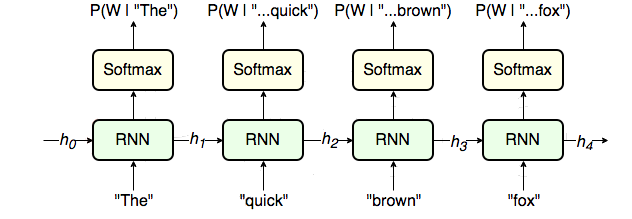
\includegraphics[width=\textwidth]{figures/rnn_language_model.png}

\end{frame}

\begin{frame}{Modèles de langue}

\begin{description}
	\item [Exemple] Modèle de langue imitant \textbf{Shakespeare} \cite{karpathy2015unreasonable}
\end{description}

\begin{quote}
{\small
PANDARUS:\\
Alas, I think he shall be come approached and the day\\
When little srain would be attain'd into being never fed,\\
And who is but a chain and subjects of his death,\\
I should not sleep.\\ \vspace{.5cm}

Second Senator:\\
They are away this miseries, produced upon my soul,\\
Breaking and strongly should be buried, when I perish\\
The earth and thoughts of many states.\\ \vspace{.5cm}

DUKE VINCENTIO:\\
Well, your wit is in the care of side and that. }
\end{quote}

\end{frame}

\begin{frame}{Modèles de langue}
\begin{description}
	\item [Exemple] Modèle de langue imitant des articles de géométrie algébrique en \LaTeX \cite{karpathy2015unreasonable}
\end{description}

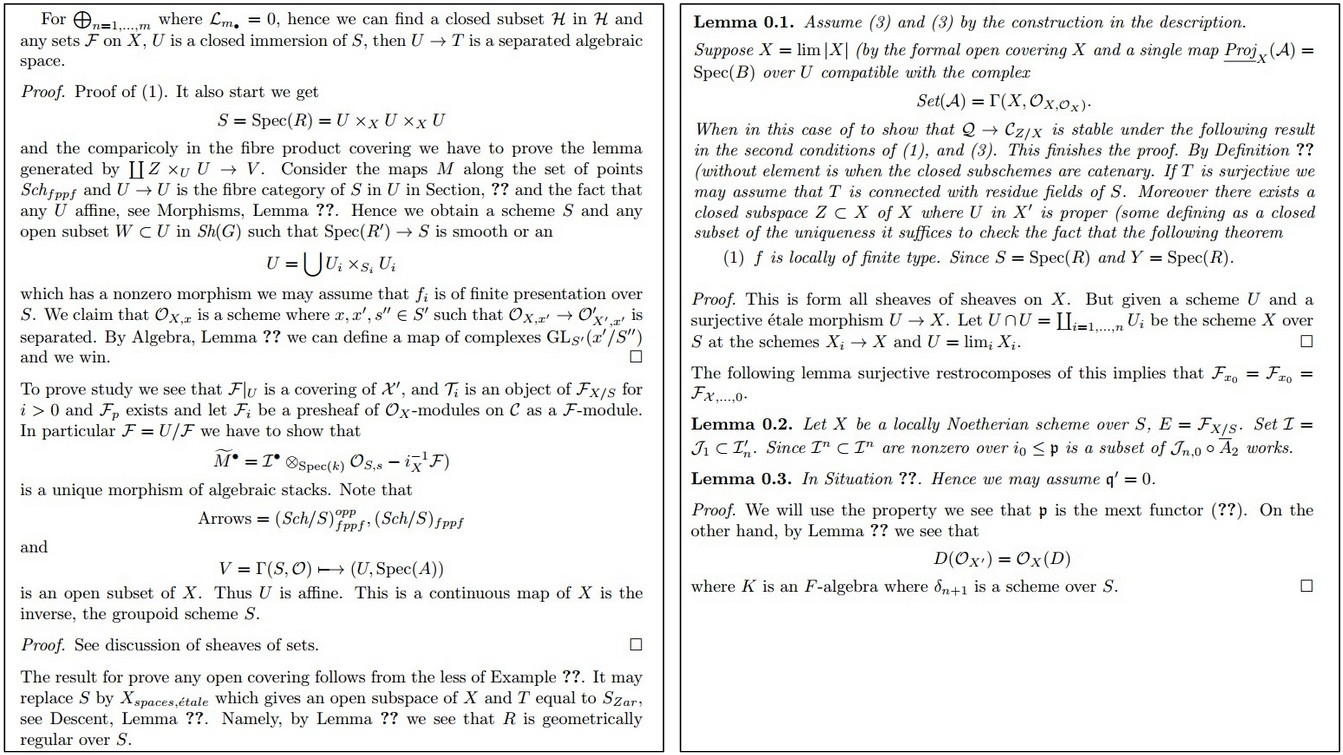
\includegraphics[width=\textwidth]{figures/latex_rnn}

\end{frame}

% Neural Machine Translation

\subsection{Traduction automatique}

\begin{frame}{Traduction automatique}

\begin{description}
	\item [Tâche] Traduire une phrase d'une langue source vers une langue cible.
\end{description}

Approche simple :
\begin{itemize}
	\item On utilise un modèle Seq2Seq.
	\item On utilise des word embeddings pour représenter les mots.
\end{itemize}
\centering
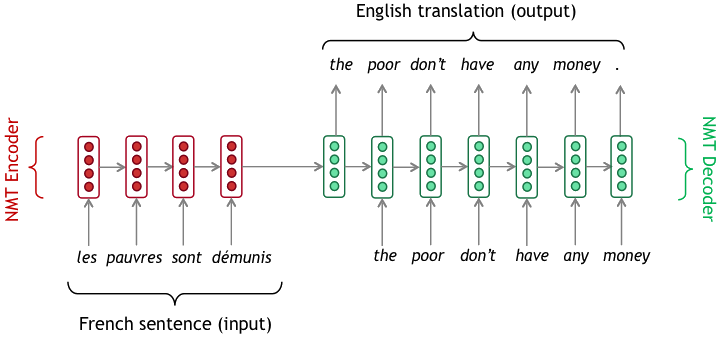
\includegraphics[width=0.8\textwidth]{figures/seq2seq_machine_translation}
\end{frame}

\begin{frame}{Traduction automatique}

\begin{description}
	\item [Exemple] Traduction anglais vers français \cite{sutskever2014sequence}
\end{description}
\vspace{.5cm}
\begin{itemize}
	\item \textbf{Traduction générée} : Avec la crémation , il y a un " sentiment de violence contre le corps d ' un être cher " , qui sera " réduit à une pile de cendres " en très peu de temps au lieu d ' un processus de décomposition " qui accompagnera les étapes du deuil " .

	\item \textbf{Cible} : Il y a , avec la crémation , " une violence faite au corps aimé " , qui va être " réduit à un tas de cendres " en très peu de temps , et non après un processus de décomposition , qui " accompagnerait les phases de deuil " .
\end{itemize}

\begin{description}
	\item [Limitations] Toute l'information contenue dans la phrase source est transmise au décodeur par un seul vecteur de taille fixe. Les modèles ont alors tendance à avoir de la difficulté à traduire de longues phrases.
\end{description}

\end{frame}

\begin{frame}{Traduction automatique}

\centering
{\Large Solution : \textbf{Mécanisme d'attention} \cite{bahdanau2014neural}}
\begin{columns}[T] % align columns
\begin{column}{.45\textwidth}

\vspace{2cm}
\begin{itemize}
	\item Le modèle apprend à aligner les mots de la phrase d'entrée avec ceux de la phrase de sortie.
\end{itemize}

\end{column}%
\hfill%
\begin{column}{.55\textwidth}
\centering
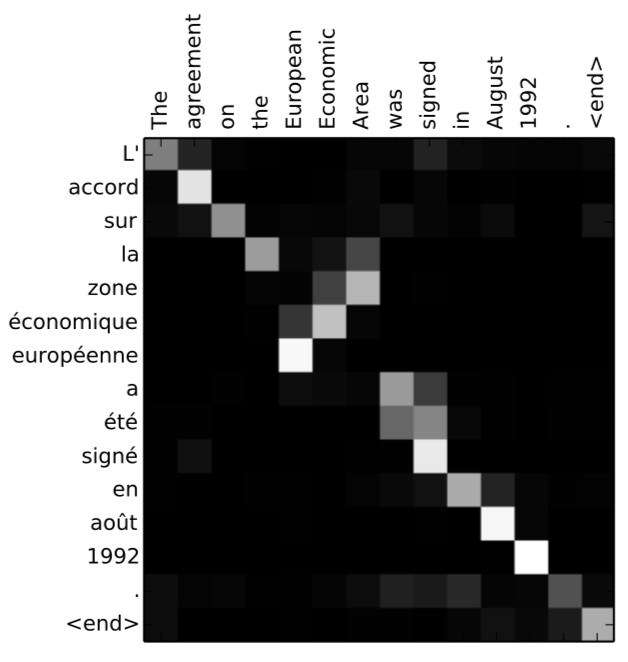
\includegraphics[width=\textwidth]{figures/attention_visualisation}
\end{column}%
\end{columns}

\end{frame}

% Conversational Agents

\subsection{Agents conversationnels}

\begin{frame}{Agents conversationnels}

\begin{itemize}
	\item Communément appelés \textit{chatbots}
	\item Tâche similaire à la traduction automatique. 
\end{itemize}

Test de Turing \cite{turing2009computing} :
\begin{itemize}
	\item Le but de A est de tromper l'interrogateur (C).
	\item Le but de B est d'aider C.
	\item Si une machine remplace A, puis C prédit à 50\% qui est qui, le test est passé.
\end{itemize}

\centering
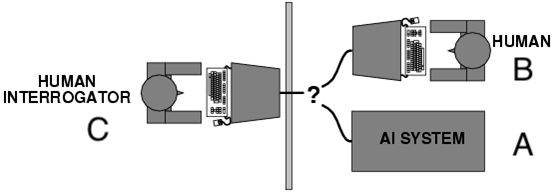
\includegraphics[width=0.7\textwidth]{figures/turing_test}

\end{frame}

\begin{frame}{Agents conversationnels}
\begin{description}
	\item [Exemple] Réponses générées par un modèle Seq2Seq simple \cite{vinyals2015neural}
\end{description}
\vspace{-.3cm}
\begin{columns}[T] % align columns
\begin{column}{.48\textwidth}

\begin{description}
	\item [Human] hello !
	\item [Machine] hello !
	\item [Human] how are you ?
	\item [Machine] i ’m good .
	\item [Human] what ’s your name ?
	\item [Machine] i ’m julia .
	\item [Human] when were you born ?
	\item [Machine] 1977 .
\end{description}

\end{column}%
\hfill%
\begin{column}{.58\textwidth}
\begin{description}
	\item [Human] where are you from ?
	\item [Machine] i ’m out in the boonies.
	\item [Human] are you a man or a woman ?
	\item [Machine] i ’m a woman .
	\item [Human] why are we here ?
	\item [Machine] i ’m not sure .
	\item [Human] okay, bye !
	\item [Machine] bye .
\end{description}
\end{column}%
\end{columns}

\vspace{.3cm}
Difficultés : 

\begin{itemize}
	\item Les réponses générées sont courtes et peu originales.
	\item L'agent conversationnel n'a pas de personnalité cohérente.
\end{itemize}
\end{frame}

\begin{frame}{Conclusion}

\vspace{.3cm}
Introduction à divers modèles neuronaux utilisés dans le NLP :
\begin{itemize}
	\item MLP, RNN, Seq2Seq
\end{itemize}
\vspace{.3cm}
Différentes façons de représenter les mots :
\begin{itemize}
	\item Bag of Words, Word Embeddings
\end{itemize}
\vspace{.3cm}
Présentation de quelques tâches en NLP :
\begin{itemize}
	\item Analyse de sentiments, Modèles de langue, Traduction automatique, Chatbots
\end{itemize}
\end{frame}

\begin{frame}{Pour aller plus loin...}

Blog posts informatifs sur le NLP et l'apprentissage profond:
\begin{itemize}
	\item \href{http://karpathy.github.io/2015/05/21/rnn-effectiveness/}{Karpathy : The Unreasonable Effectiveness of Recurrent Neural Networks}
	\item \href{http://colah.github.io/posts/2015-08-Understanding-LSTMs/}{Olah : Understanding LSTM Networks}
	\item \href{https://machinelearningmastery.com/gentle-introduction-bag-words-model/}{Brownlee : A Gentle Introduction to the Bag-of-Words Model}
	\item \href{https://machinelearningmastery.com/what-are-word-embeddings/}{Brownlee : What Are Word Embeddings for Text?}
	\item \href{https://pytorch.org/tutorials/intermediate/seq2seq_translation_tutorial.html}{Robertson : Translation with a Sequence to Sequence Network and Attention}
\end{itemize}

\vspace{.3cm}
Librairies Python pour le NLP et l'apprentissage profond:
\begin{itemize}
	\item \href{https://www.nltk.org/}{Natural Language Tool Kit (NLTK)}
	\item \href{https://pytorch.org/}{PyTorch}
	\item \href{http://opennmt.net/OpenNMT-py/}{OpenNMT-Py}
\end{itemize}

\end{frame}

\section*{Références}

\begin{frame}[t,allowframebreaks]
\setbeamertemplate{bibliography item}{[\theenumiv]}


  \frametitle{Références}
  \nocite*
  \bibliographystyle{siam}
  \bibliography{references}
 \end{frame}

\end{document}